%----------------------------------------------------------------------------
\appendix
%----------------------------------------------------------------------------
\chapter*{\fuggelek}\addcontentsline{toc}{chapter}{\fuggelek}
\setcounter{chapter}{\appendixnumber}
%\setcounter{equation}{0} % a fofejezet-szamlalo az angol ABC 6. betuje (F) lesz
\numberwithin{equation}{section}
\numberwithin{figure}{section}
\numberwithin{lstlisting}{section}
%\numberwithin{tabular}{section}

%----------------------------------------------------------------------------
%\section{A TeXstudio felülete}
%----------------------------------------------------------------------------
%\begin{figure}[!ht]
%\centering
%\includegraphics[width=150mm, keepaspectratio]{figures/TeXstudio.png}
%\caption{A TeXstudio \LaTeX-szerkesztő.} 
%\end{figure}

%----------------------------------------------------------------------------
%\clearpage\section{Válasz az ,,Élet, a világmindenség, meg minden'' kérdésére}
%----------------------------------------------------------------------------
%A Pitagorasz-tételből levezetve
%\begin{align}
%c^2=a^2+b^2=42.
%\end{align}
%A Faraday-indukciós törvényből levezetve
%\begin{align}
%\rot E=-\frac{dB}{dt}\hspace{1cm}\longrightarrow \hspace{1cm}
%U_i=\oint\limits_\mathbf{L}{\mathbf{E}\mathbf{dl}}=-\frac{d}{dt}\int\limits_A{\mathbf{B}\mathbf{da}}=42.
%\end{align}


%installation, futtatas
%mi van a zpi mellekletben
%mellekletben tesztesetek

The source code of the symbolic execution tool and the tested VIs are included in the attachment of this BSc thesis. 

\paragraph{Contents of the attachment:}
\begin{itemize}
\item SymbolicTool: Source code of the tool
\item Test VIs

\begin{itemize}
\item Demo\textunderscore A.gvi: The example VI of Demo A
\item Demo\textunderscore B.gvi: The example VI of Demo B
\item Test\textunderscore C.gvi: VI with no case structures
\item Test\textunderscore D.gvi: A more complex example introducing mixed types of input data
\item Test\textunderscore E.gvi: An example on solving for multiplication
\item Test\textunderscore F.gvi: Testing for a 4-variable logical function

\end{itemize}
\end{itemize}
\section{Installation and run}

Before installation, make sure, the system meets the hardware requirements of LabVIEW NXG\footnote{\url{http://www.ni.com/hu-hu/shop/labview/compare-labview-nxg-and-labview.html}}.
\paragraph{Recommended software environment:}
\begin{itemize}
\item Microsoft Windows 7 / 8.1 / 10\footnote{\url{https://www.microsoft.com/en-us/windows}}
\item Microsoft .NET framework 4.6.2\footnote{\url{https://www.microsoft.com/en-us/download/details.aspx?id=53344}}
\item Microsoft Visual Studio 15\footnote{\url{https://visualstudio.microsoft.com/vs/}}
\item Microsoft Research Z3 Solver\footnote{\url{https://www.microsoft.com/en-us/download/details.aspx?id=52270}}
\item National Instruments LabVIEW NXG 2.1\footnote{\url{http://www.ni.com/en-us/shop/labview/labview-nxg.html}}
\end{itemize}
Open solution \verb|SymbolicTool.sln| with Visual Studio. After opening the project, the paths of referenced libraries might need to be adjusted to the paths on the actual system. 

After building, copy \verb|SymbolicTool.plugin.dll| from the \verb|bin| folder of the project to the \verb|Addons| folder of \verb|LabVIEW NXG 2.1| (or a sub-folder). Copying Z3 libraries to the \verb|Addons| folder might also be necessary. Run LabVIEW. A new entry called SymbolicTool should appear in the main menu bar. Select the commands of this menu, when a Block Diagram of a VI is active on the screen.
\begin{figure}
\centering
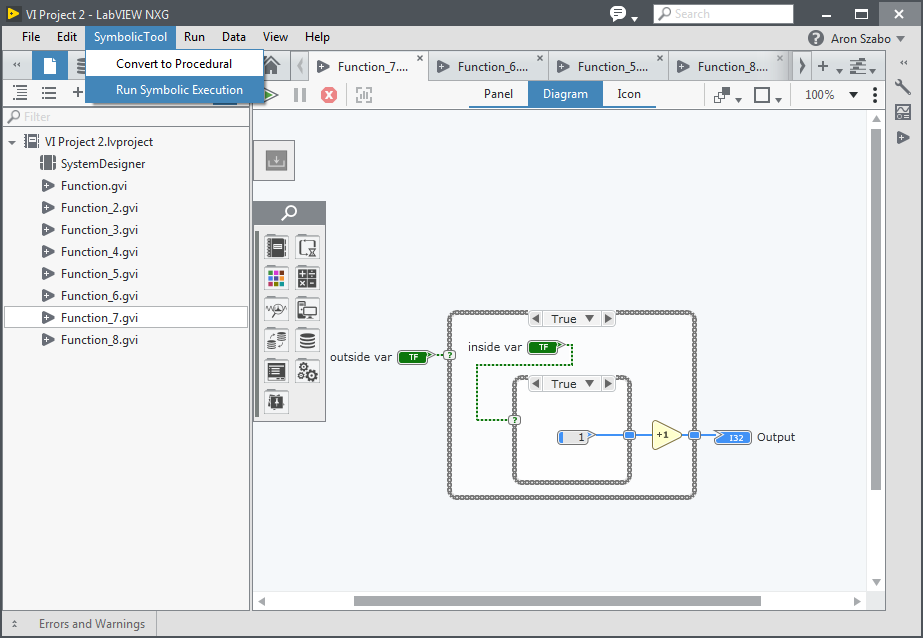
\includegraphics[width=150mm,keepaspectratio]{figures/interface.png}
\caption{Interface of LabVIEW NXG 2.1 with SymbolicTool installed} 
\label{fig:interface1}
\end{figure}

\paragraph{Debugging} Copy \verb|SymbolicTool.plugin.pdb| to the \verb|Addons| folder along with the DLL. Run LabVIEW and open a project. Select Debug / Attach to process... in Visual Studio and attach to \verb|LabVIEW NXG.exe|. Now the debugger in Visual Studio can be used.
